\section{Results}
%\subsection{General results}
%
%After excluding faulty cameras we had TK cameras in total, 19 in the Control-group and 33 in the experiment group.
%A total of TK photos were taken, of whom TK contained photos of the species I've focused on in my study. Check table for more details.
%
%The species I've focused on was mainly night-active as displayed in the density plots \ref{fig:overlap}, (with the exception of squirrel). In other words, all of them experienced a white LED flash during night hours.
%(Caption: Figure is split up in periods with and without white LED flash. Night activity in the dashed curve highlights the times the species would have experienced the flash. "Carpet"-below the curves signifies datapoints of each "group".
%



\subsection{GLMM}
Results of the roe deer.

Model formula: n.obs ~ time.deploy + flash + (1|loc) + (1|week)

I fitted a poisson mixed model (estimated using ML and Nelder-Mead optimizer) to predict n.obs with time.deploy and flash (formula: n.obs ~ time.deploy * flash).
The model included loc and week as random effects (formula: list(~1 | loc, ~1 | week)).
The model's total explanatory power is substantial (conditional R2 = 0.45) and the part related to the fixed effects alone (marginal R2) is of 1.95e-03.
The model's intercept, corresponding to time.deploy = 0 and flash = 0, is at -3.38 (95\% CI [-3.97, -2.78], p < .001).


Standardized parameters were obtained by fitting the model on a standardized version of the dataset. 95\% Confidence Intervals (CIs) and p-values were computed using the Wald approximation. Predicted counts visualised in \vref{fig:glmm_sp}, model parameters visualised in \vref{fig:para_sp}.


\begin{figure}
		\begin{subfigure}{.5\textwidth}
		  \centering
		  	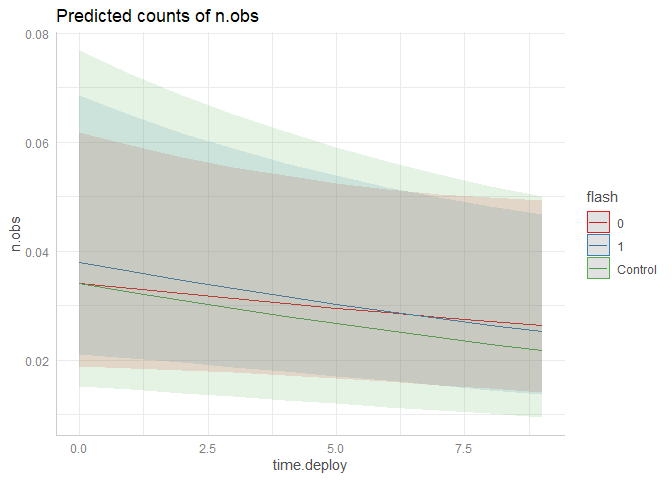
\includegraphics[width=.8\linewidth]{../R/glmm_sp_files/figure-gfm/raadyr-C-report-1.png}
		  \caption{Roe deer}
		  	\label{fig:glmm_raa}
	\end{subfigure}
		\begin{subfigure}{.5\textwidth}
		  \centering
		  	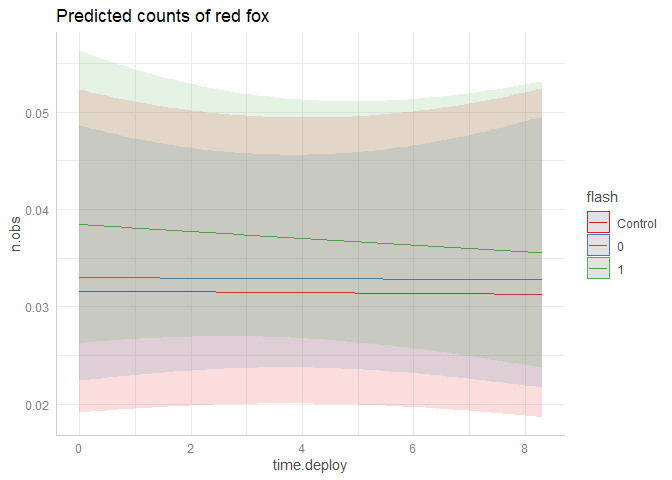
\includegraphics[width=.8\linewidth]{../R/glmm_sp_files/figure-gfm/rev-report-1.png}
		  \caption{Red fox}
		  	\label{fig:glmm_rev}
	\end{subfigure}
		\begin{subfigure}{.5\textwidth}
		  \centering
		  	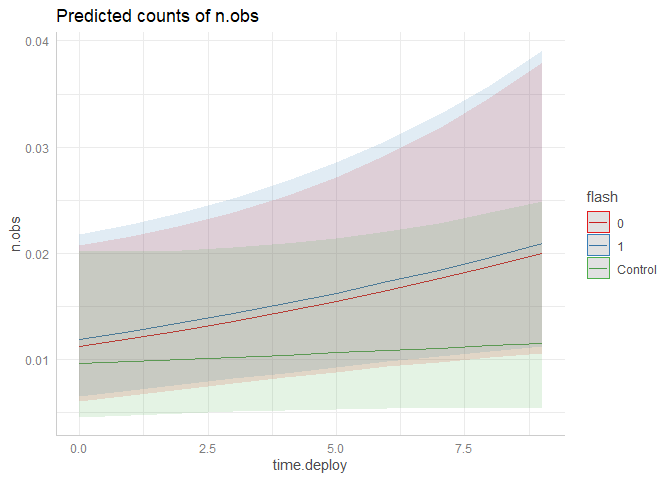
\includegraphics[width=.8\linewidth]{../R/glmm_sp_files/figure-gfm/grevling-report-1.png}
		  \caption{Badger}
		  	\label{fig:glmm_grvl}
	\end{subfigure}
		\begin{subfigure}{.5\textwidth}
		  \centering
		  	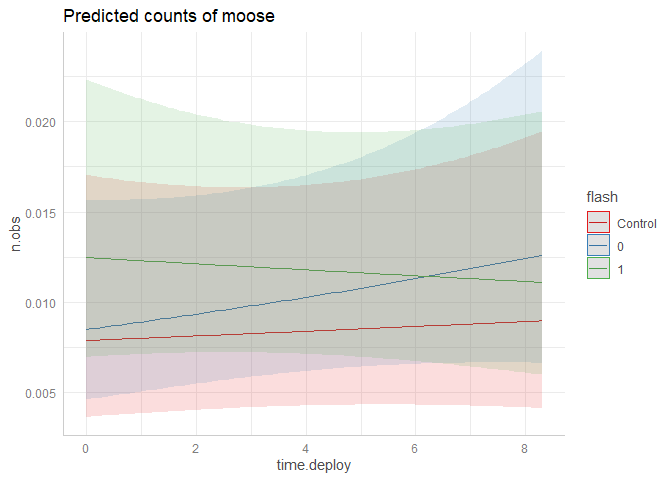
\includegraphics[width=.8\linewidth]{../R/glmm_sp_files/figure-gfm/elg-report-1.png}
		  \caption{Moose}
		  	\label{fig:glmm_elg}
	\end{subfigure}
		\begin{subfigure}{.5\textwidth}
		  \centering
		  	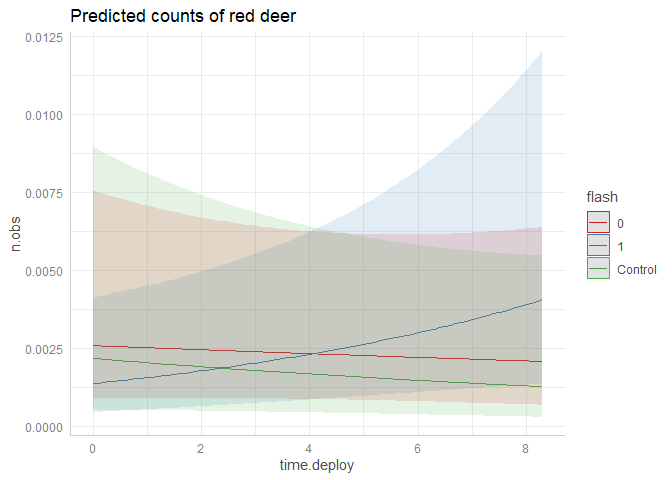
\includegraphics[width=.8\linewidth]{../R/glmm_sp_files/figure-gfm/hjort-report-1.png}
		  \caption{Red deer}
		  	\label{fig:glmm_hjort}
	\end{subfigure}
		\begin{subfigure}{.5\textwidth}
		  \centering
		  	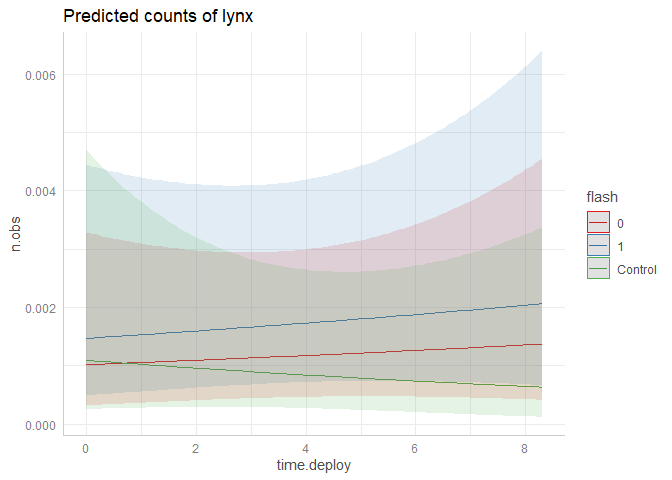
\includegraphics[width=.8\linewidth]{../R/glmm_sp_files/figure-gfm/gaupe-report-1.png}
		  \caption{Lynx}
		  	\label{fig:glmm_gaup}
	\end{subfigure}
		\caption{Fitted GLMM model to each species}
	\label{fig:glmm_sp}
\end{figure}




\begin{figure}
		\begin{subfigure}{.4\textwidth}
		  \centering
	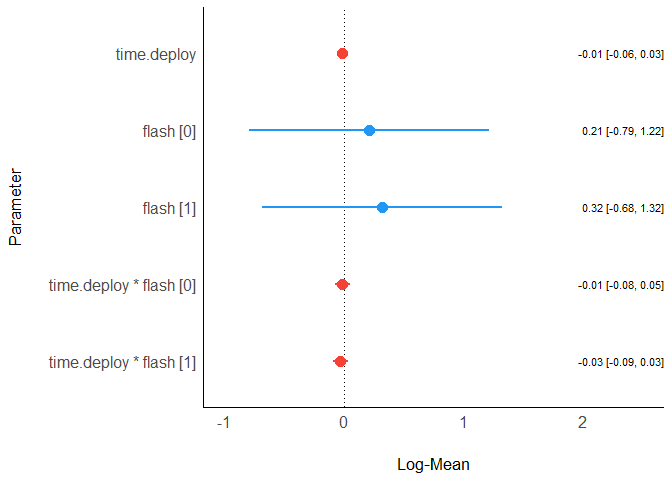
\includegraphics[scale=.4]{../R/glmm_sp_files/figure-gfm/parameters-1.png}
\caption{Intercept included}
		\label{fig:para_raa1}
	\end{subfigure}
		\begin{subfigure}{.4\textwidth}
		  \centering
	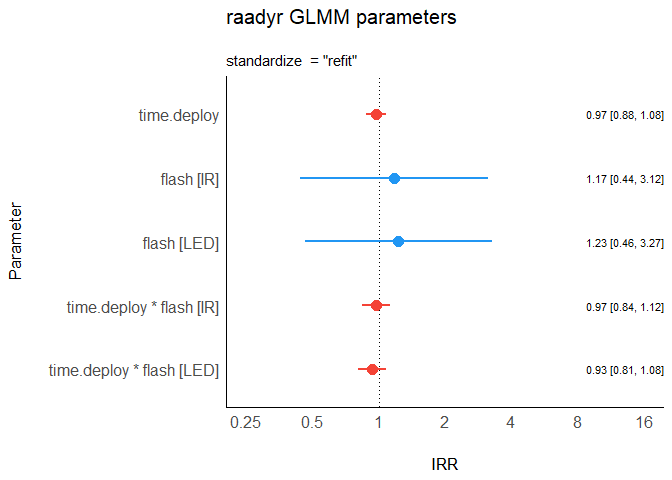
\includegraphics[scale=.4]{../R/glmm_sp_files/figure-gfm/parameters-2.png}
\caption{with values printed}
		\label{fig:para_raa2}
	\end{subfigure}
		\begin{subfigure}{.8\textwidth}
		  \centering
	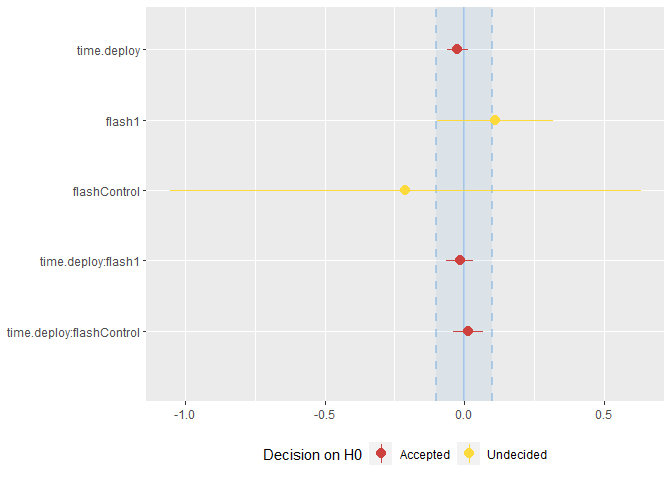
\includegraphics[scale=1]{../R/glmm_sp_files/figure-gfm/parameters-3.png}
\caption{Equivalence test}
		\label{fig:para_raa3}
	\end{subfigure}
		\caption{Visualising model parameters}
	\label{fig:para_sp}
\end{figure}




\subsection{Kommentar}

Så langt har eg fokusert på rådyr, men nå er det ikkje så mykje arbeid å skrive vidare om resten av artene.

Planen er å lage eit felles plot i stil med eit av plottene i figur \ref{fig:para_sp}. Då vil kvar art få kvart sitt konfidensintervall (CI) for kvar parameter.
Dei to øverste er vanlige effect size-plot, det nederste er omformulert til ein ekvivalens-test som baserer seg på bayesisk statistikk, kor man kan akseptere nullhypoteser, ikkje berre avslå eller feile i å avslå.

Det er kanskje ikkje heilt naudsynleg å ta med, sidan eg ikkje har gjort bayesiske analyser, men den har blitt modifisert til frekventist-analyser også, og det er slik eg bruker den.
Den oppfører seg som ein kommentar til / visualisering av p-testen. Vis parameter-effekten har heile CI sitt inni ROPE-området kan man "akseptere" nullhypotesen, uansett om p-verdien seier den er signifikant. Vis CI tangerer ROPE området kan man ikkje konkludere angåande parameteret. For meg resulterer begge disse tilfellene i at eg feiler med å avslå nullhypotesen.

Til slutt, vis CI er heilt utanfor ROPE-området, er effekten signifikant (p < 0.5) og eg kan avslå nullhypotesen.


Kva for ein variant av plottene synest du viser modellen best?





\subsection{CPH mixed effect}
%n.obs ~ time.deploy + flash*species + random.eff
%report::report()?
%
%
%\subsection{H2 test}
%house\_d2 eller ALAN\_d2
%report::report()
%






